\documentclass{beamer}
\usepackage{tikz}

\usetheme{metropolis}           % Use metropolis theme

\title{Securing IoT Networks through Moving Target Defence}
\subtitle{CSCS25}            % ← conference name as subtitle

\date{May 28, 2025}
\author{%
  Andrei Vlădescu\inst{1} \and
  Prof.\ Dr.\ Ion Bica\inst{2}
}
\addtobeamertemplate{title page}{
  \begin{tikzpicture}[remember picture,overlay]
    \node[anchor=north east, xshift=0.1cm, yshift=-6.9cm]
      at (current page.north east)
      {
\includegraphics[height=2.5cm]{images/logo_upb.png}};
  \end{tikzpicture}
}{}

\institute[UNSTV]{%                            % ← short institute in square brackets
  \inst{1} University Politehnica of Bucharest (UPB)\\
  \inst{2} “Ferdinand I” Military Technical Academy
}

\begin{document}

\maketitle

% Outline
\begin{frame}{Outline}
  \tableofcontents
\end{frame}

% 1. Introduction
\section{Introduction}

\begin{frame}{Context \& Motivation}
  \begin{itemize}
    \item Explosion of IoT devices in smart homes, healthcare, critical infrastructure
    \item Resource constraints \& lack of built-in security 
    \item IoT as attractive targets for large-scale DDoS attacks
  \end{itemize}
\end{frame}

\begin{frame}{Research Objectives}
  \begin{itemize}
    \item Evaluate Moving Target Defence (MTD) for IoT security
    \item Integrate MTD with Software-Defined Networking (SDN)
    \item Evaluate the solution in a public network
  \end{itemize}

  \note{}
\end{frame}

% 2. Technical Primer
\section{Technical Primer}

\begin{frame}{Moving Target Defense (MTD)}
  \begin{itemize}
    \item Dynamically alters attack surface  
    \item Examples: ASLR, ISR, honeypots/honeynets  
    \item Increases attacker uncertainty and cost  
  \end{itemize}
\end{frame}

\begin{frame}{Software-Defined Networking (SDN)}
  \begin{itemize}
    \item Separation of control plane (controller) and data planes (switches)  
    \item Northbound API: apps → controller  
    \item Southbound API: controller → forwarding devices  
  \end{itemize}
\end{frame}

\begin{frame}{State-of-the-Art \& Where We Fit}
\begin{itemize}
    \item \textbf{Mutable Networks (MUTE)} – crypto-shuffled IP/port mapping
    \item \textbf{Random Host Mutation (RHM)} – edge IP shuffling
    \item \textbf{OF-RHM (OpenFlow)} – SDN-based randomization
  \end{itemize}
\end{frame}

% 3. Proposed Architecture
\section{Proposed Architecture}

\begin{frame}{Threat Model}
  \begin{itemize}
    \item Botnet-driven volumetric DDoS (SYN/UDP flooding)  
    \item Target: resource-constrained IoT devices (no IDS/ACL)
    \item Reconnaissance \& Exploitation threat vectors also considered
  \end{itemize}
\end{frame}

\begin{frame}{System Architecture}
  \begin{center}
    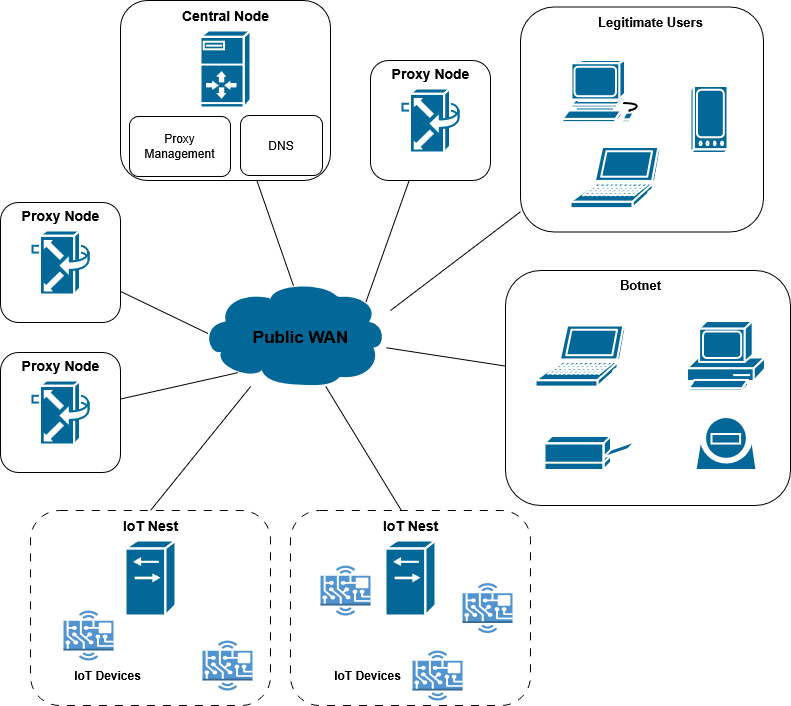
\includegraphics[width=0.83\textwidth]{presentation/images/system_architecture.png}
  \end{center}
  
\end{frame}

\begin{frame}{Defence Workflow}
  \begin{center}
    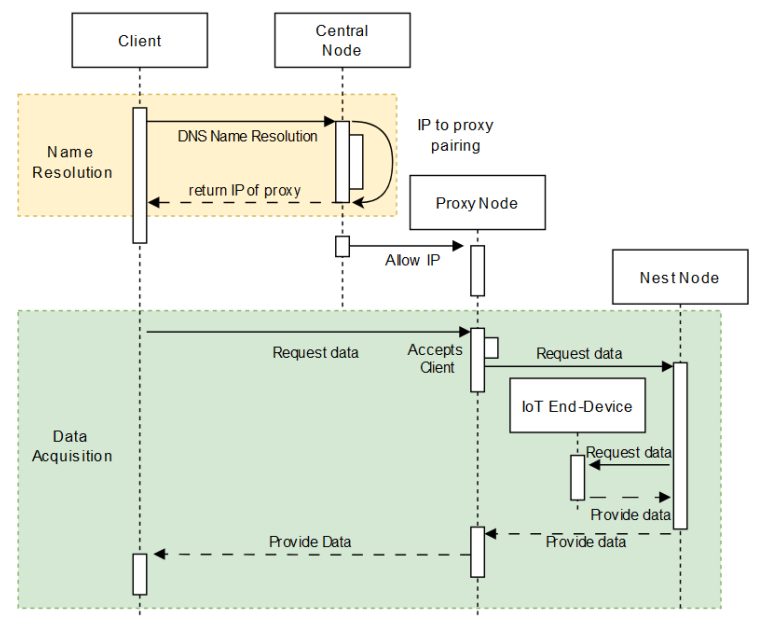
\includegraphics[width=0.83\textwidth]{presentation/images/sequence_diagram.png}
  \end{center}
\end{frame}

\begin{frame}{Defence Workflow}
Case I - Botnet is not connected
    \begin{enumerate}
        \item Recon is done to find the IP address of the proxy
        \item Botnet floods directly to the IP
        \item Botnet is blocked by the proxy
    \end{enumerate}

\end{frame}

\begin{frame}{Defence Workflow}
Case II - Botnet is connected
    \begin{enumerate}
        \item Bots flood the IPs of the proxies assigned to them
        \item Proxy will detect the flood and flag the IPs
        \item Master Node will renew the IP address of the proxies from the ISP's DHCP server
        \item Legitimate users will be able to connect again to the DNS
    \end{enumerate}

\end{frame}

% 4. Results & Insights
\section{Results \& Insights}

\begin{frame}{Simulation Environment}
  \begin{itemize}
    \item Simulated Internet inside VMs and Docker
    \item ESP8266 microcontroller HTTP service
    \item Locust framework \& Ixia Breakingpoint for traffic generation
    \item Power usage measurement using a lab bench power supply
    \item Scenarios: baseline, nominal load, volumetric DDoS  
  \end{itemize}
\end{frame}

\begin{frame}{Simulation Environment}
    Ixia Breakingpoint Data Rate Curve
    \vspace{1em}
    \begin{center}
        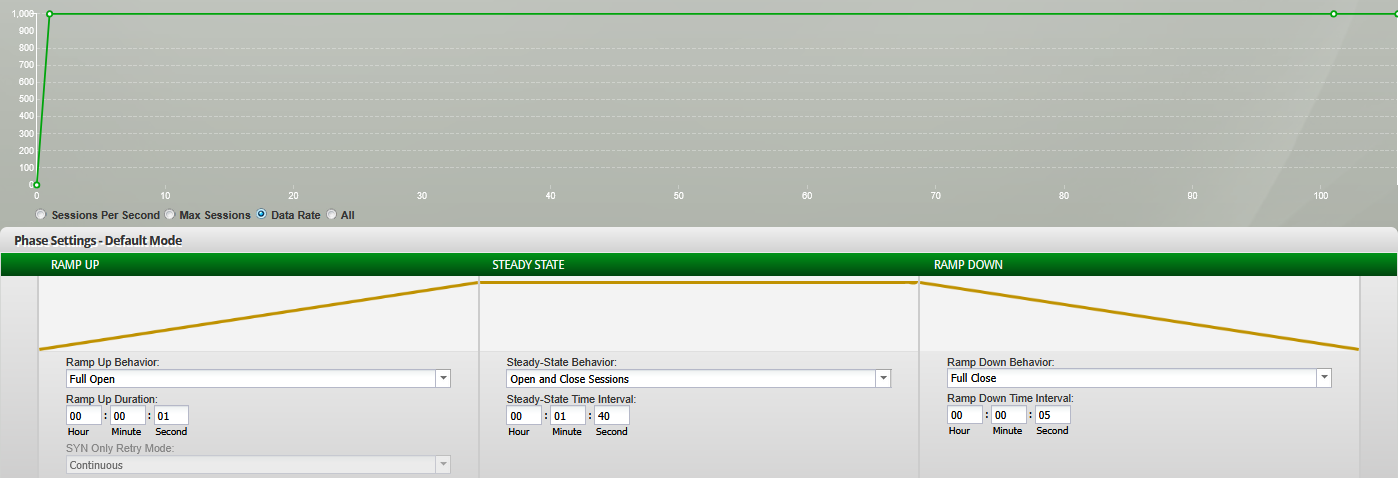
\includegraphics[width=\textwidth]{images/breakingpoint_curve.png}
    \end{center}
\end{frame}

\begin{frame}{Evaluation Metrics}
  \begin{itemize}
    \item \textbf{Latency} 
    \item \textbf{Failure Rate}
    \item \textbf{Power Usage}
  \end{itemize}
\end{frame}


\begin{frame}{Statistics}
    Nominal Usage
    \vspace{1em}
    \begin{center}
        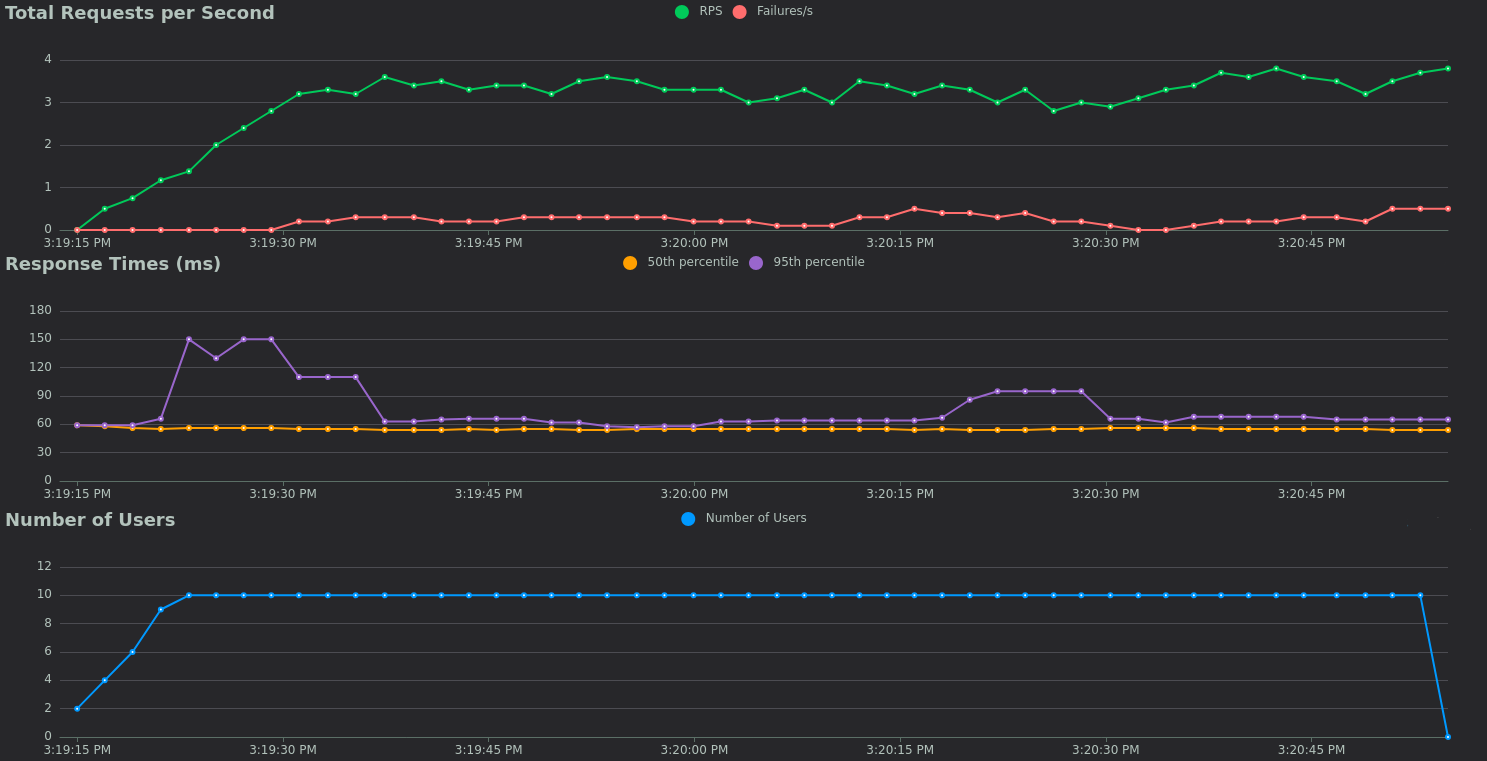
\includegraphics[width=\textwidth]{images/nominal_usage.png}
    \end{center}
\end{frame}

\begin{frame}{Statistics}
    Unprotected Attack
    \vspace{1em}
    \begin{center}
        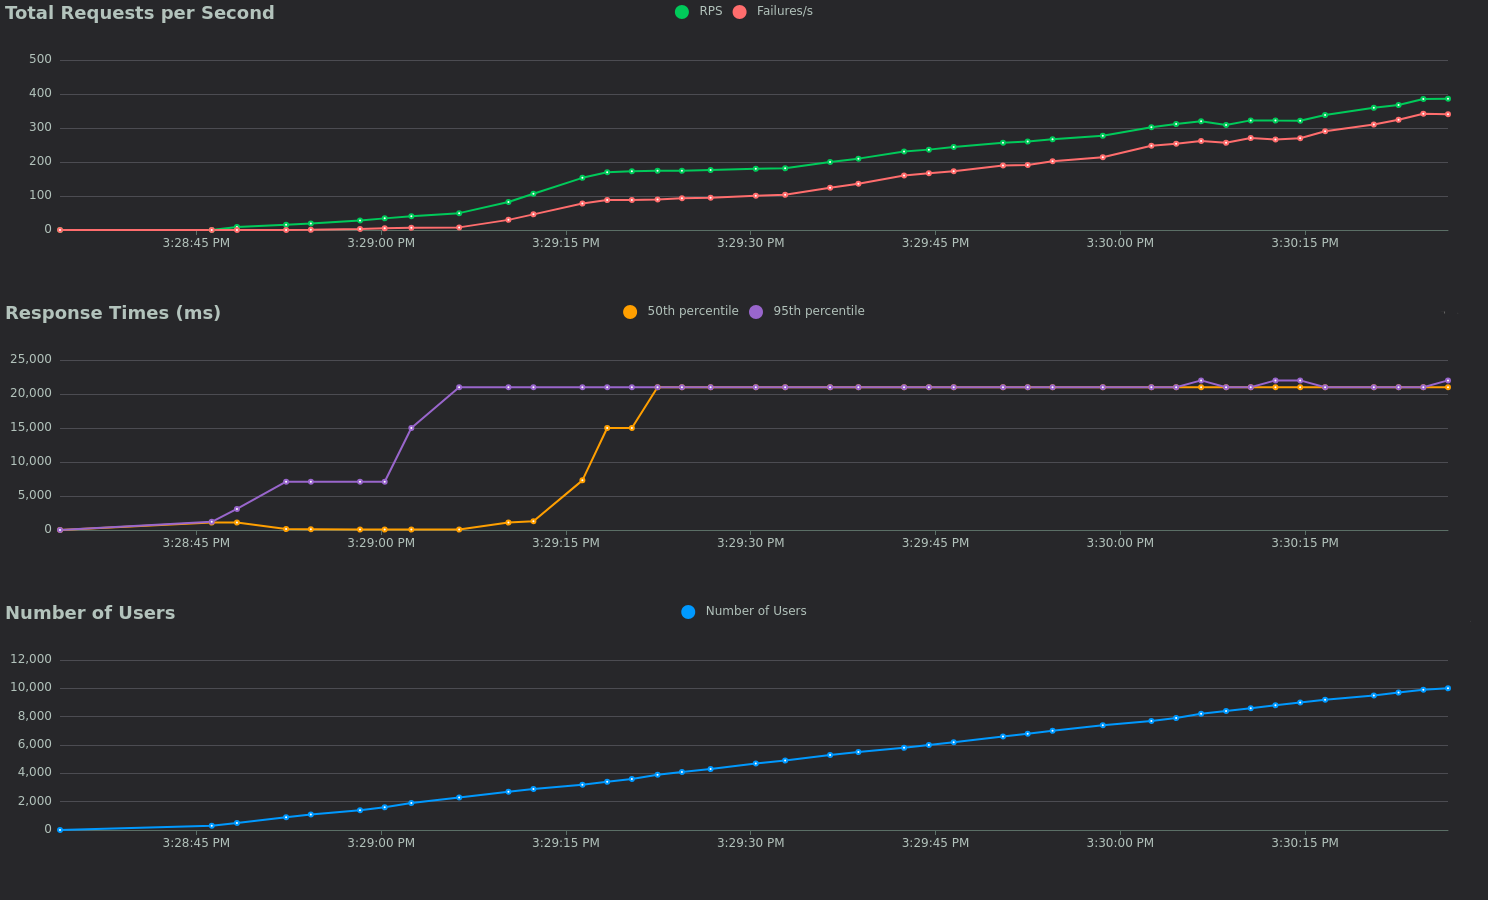
\includegraphics[width=\textwidth]{images/ddos_usage.png}
    \end{center}
\end{frame}

\begin{frame}{Statistics}
Power Draw
    \vspace{1em}

  \begin{center}
    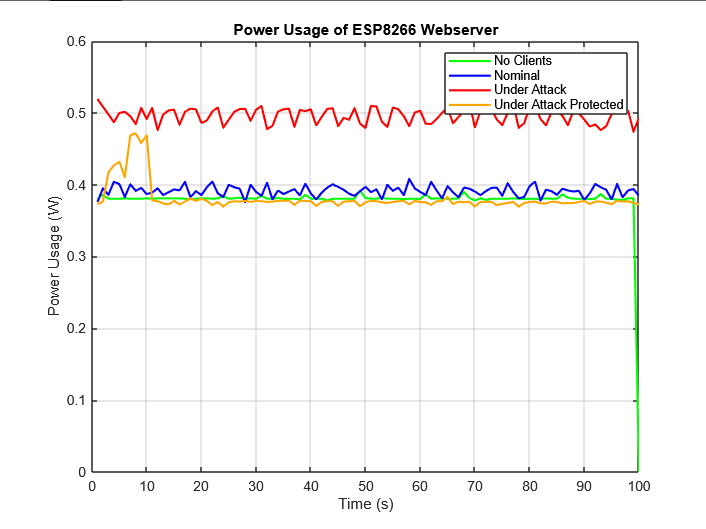
\includegraphics[width=0.8\textwidth]{images/power_usage_esp8266.png}
  \end{center}
\end{frame}

\begin{frame}{The Good, the Bad \& the Lag}
  \begin{itemize}
    \item \textbf{Advantages}:
      \begin{itemize}
        \item Cheap-ish
        \item Increases attacker cost
        \item Easy to implement in public WAN networks
        \item Modular, device agnostic approach
      \end{itemize}
    \item \textbf{Limitations}:
      \begin{itemize}
        \item Overhead from ISP IP changes is a wildcard
        \item Needs complementary security measures
        \item Will need to be fine tuned for different services
      \end{itemize}
  \end{itemize}
\end{frame}


%\begin{frame}{Future Work}
%  \begin{itemize}
%    \item Integrate ML-based DDoS detection  
%    \item Test in real-world ISP networks  
%    \item Explore IPv6-only deployments  
%  \end{itemize}
%\end{frame}

% Q&A
\begin{frame}{Q\&A}
  \centering Thank you!\par
  \vspace{1em}
  \large Any questions?
\end{frame}

\end{document}
